\documentclass[10pt, compsoc, conference]{IEEEtran}

\usepackage{etoolbox}
\usepackage{graphicx}
\usepackage[style=numeric,sorting=none]{biblatex}

% remove \centering from \section
\patchcmd{\section}{\centering}{}{}{}

\addbibresource{references.bib}

\begin{document}
\title{ARIMA Analysis of Risk in \\Open-Source Project Dependencies}

\author{\IEEEauthorblockN{Róisín Ní Bhriain}
\IEEEauthorblockA{Student Number: 23269640}
\and
\IEEEauthorblockN{Sneha Dechamma Mallengada Suresh}
    \IEEEauthorblockA{Student Number: 23262168}}

\maketitle

\vspace*{-1.5234cm}

\thispagestyle{plain}
\pagestyle{plain}

\begin{description}
    \item[]
    \begin{center}
        %\item[\textbf{Technical Manual}] 
        \end{center}
    \item[]
\end{description}


\begin{abstract}
Measuring risk is essential in ensuring the security, reliability and compliance in software systems. Open-source software is transparent and accessible to everyone but can be vulnerable to security risks and thus requires analysis to identify and mitigate against these risks. Developers and organisations need to understand the risks associated with their open-source supply chain to safeguard against any data breaches or other attacks. Making informed decisions on software adoption by comparing the risks in different components is a part of this. This paper explores the methods used in the prediction of risk when using open-source software. There are a number of methods used and the aim is to combine these to give a more comprehensive view of the risks of using a particular open-source project. We examine the literature to decide on an appropriate prediction algorithm for each section. We aim to develop a tool to investigate the risks in dependency trees. We provide a graph of the final results which can be used to aid in finding where the risk lies in the dependency trees. 
\end{abstract}

\begin{IEEEkeywords}
ARIMA prediction, software vulnerabilities, Maven.
\end{IEEEkeywords}

\section{Introduction}
The popularity of open-source software in large software projects has increased in the last number of years \cite{zajdel_open_2022}. The reuse of libraries can reduce development efforts substantially for developers. In particular, the use of open-source libraries is unrestricted and transparent which means developers can modify and distribute the code to their needs. The reuse of libraries can create a list of dependencies called a supply chain. The supply chain is a chain of dependencies, which can include open-source software. The supply chain involves a network of participants who perform activities on the dependencies \cite{k_singi_trusted_2019}. As software projects grow larger so do the supply chains and thus they can become difficult to manage leading developers to turn to package managers. In Java in particular the average application depends on about 40 third-party libraries \cite{a_m_mir_effect_2023}. 

With the increased use of open-source software, attackers have begun to exploit known vulnerabilities in trusted components in the supply chains by injecting malicious code into software packages \cite{ohm_backstabbers_2020}. These types of attacks are set to increase with 34\% of all recorded supply chain attacks taking place in 2020 and 66\% of all recorded supply chain attacks occurring in 2021 \cite{m_z_malik_protection_2023}. These attacks can come at a great cost to users of open-source software with data breaches in particular coming at a cost of \$388 million on average for a breach of 50 million data records\cite{x_wang_feasibility_2021}. Once vulnerabilities are discovered, it is important that users of open-source software identify whether they are impacted by the reported vulnerabilities or by inactivity in the open-source projects. 

Prediction of risk is a technique that can be used to measure whether certain open-source projects are worth using and several methods are used to predict this type of risk. Some of the key techniques in the prediction of risk in open-source software include the prediction of vulnerabilities using code metrics, the prediction of project activity on version control systems such as GitHub, and the prediction of the number of vulnerabilities released on vulnerability databases such as the National Vulnerability Database (NVD). For the purpose of this paper, we focused on the prediction of project activity and the number of vulnerabilities per month. 

This paper explores the prediction of risks in Maven dependency trees by examining both GitHub project activity and NVD vulnerability Common Vulnerabilities and Exposures (CVE) data. ARIMA prediction is used for both sets of data based on user configuration data and returns a coloured graph based on the analysed risk. The creation of a tool like this could help users identify any vulnerable components in their supply chain so they can find an alternative component which is not risky. 

The structure of this paper is as follows: we first explore the literature on the prediction of risk in open-source software focusing in particular on both project activity predictions and vulnerability predictions. We then explore some case studies where a tool to explore risk in dependency trees would have been useful for users to identify risky modules. We then describe the data from APIs that we used as well as the different predictions we made. Finally, we describe the calculations and algorithms we used when predicting risk according to user-assigned metrics and the results that we obtained. 

\section{Related Work}
In this section, we review relevant work in the prediction of risk in open-source software. We examine the machine learning models used as well as the different objects of analysis used in the predictions.  

\subsection{Vulnerability Propagation}
Only around 1.2\% of projects directly use vulnerable code in their dependencies \cite{a_m_mir_effect_2023}. However, they maintain that a small number of vulnerable projects such as \textit{jackson-databind} and \textit{netty-codec-http} can affect up to 375,607 packages in the Maven ecosystem. This means any CVEs can affect quite a large number of Maven projects. In \cite{c_liu_demystifying_2022} they create a dependency vulnerability graph of the entire NPM ecosystem. In investigating the JavaScript NPM ecosystem they propose an algorithm to resolve dependency trees as well as vulnerability propagation paths. They also find that vulnerabilities could effect up to 16.7\% of third-party libraries in their current versions. Some widely known CVEs exist at the moment in the current dependency trees of a significant number of packages. As packages grow larger and more dependencies are added the complexity of discovering vulnerable dependencies increases in complexity. The complexity can be optimised from exponential to polynomial level depending on the number of relationships through the use of a search algorithm based on lazy strategy \cite{w_hu_open_2019}. They also propose the use of optimal blocking analysis to complete vulnerability repair for a project with minimal blocking.

\subsection{Project Metadata Analysis}
Predicting project activity in open-source software is another way of measuring the success and security of projects. In \cite{l_bao_large_2021} they examine specifically the contributors in open source projects and use several machine learning and deep learning techniques to predict their activity. They attempt to differentiate between newcomers who leave the project after a short time and those who stay for a long time. Some of the most important features are the number of followers, the programming language and the average number of commits per developer. A dataset from GitHub was used as well as a survey conducted among developers to see their opinions on factors that affect long-term contributors. Predicting the health of an open-source project is explored in \cite{xia_predicting_2022}. Data from over one thousand GitHub projects was used to predict multiple health indicators using machine learning and the error rate was reduced using hyperparameter optimisation. They predict things such as the number of contributors, the number of commits, and the number of pull requests and issues. These metrics are indicative of the project’s activity level. They also conducted a survey which indicated that these are real-world concerns for developers. 

\subsection{Vulnerability CVE Data Analysis}
Time series forecasting is a popular method used when predicting vulnerabilities. In \cite{gencer_time_2021} the authors analyse the use of the ARIMA model to predict vulnerabilities. Data on vulnerabilities from the NVD was used in this study \cite{noauthor_vulnerability_nodate}. The National Vulnerability Database (NVD) is a database maintained by the National Institute for Technology which keeps updated details on known vulnerabilities. The authors aimed to predict the number of vulnerabilities for Android per month. They compared its performance with the long short-term memory model, artificial neural network and recurrent neural network deep learning techniques and found ARIMA gives better results. They found the LTSM to have comparable error rates with ARIMA and to have more successful results than the two deep learning techniques. Another paper discusses the use of ARIMA to predict vulnerabilities \cite{pokhrel_cybersecurity_2017}. They use a linear and a non-linear approach comparing ARIMA and Artificial Neural Networks ((ANN) and Support Vector Machines (SVM) again using the reported vulnerabilities on the NVD for three different Operating Systems. The results indicated that there were sharp fluctuations in the number of vulnerabilities, the non-linear approaches were a better predictor however, the ANN did not have enough data to perform well. The authors of \cite{roumani_time_2015} used two methods of time series analysis to predict vulnerabilities for web browsers: ARIMA and exponential smoothing. The trend, level and seasonality of the vulnerabilities were considered to help in prediction. They note that level was the only significant parameter. Datasets from the NVD were also used in this paper.

\section{Case Studies}
In this section, we will identify a number of case studies where a tool like this would have been valuable to see whether a project depended on a risky project. 

\subsection{Log4j}
In November 2021 a vulnerability was discovered in the popular open-source logging library Apache Log4j. This software is widely used in web portals. The vulnerability in this package means that hackers can run malicious code remotely on a victim's machine \cite{h_gupta_identification_2022}. The main aim of the log4j vulnerability is to obtain Lightweight Directory Access Protocol information and this will serve as a gateway to full control of the machine. The attack works with several steps: information gathering, weaponisation, delivery, exploitation and installation \cite{f_maulana_unmasking_2023}. A lot of projects were unaware that they were affected by the Log4j vulnerability as their dependencies relied on the Log4j library and a dependency graph of risk dependencies could have helped them discover that they were vulnerable. Once these vulnerabilities were reported a user could use the project to discover that some of their dependencies have vulnerabilities and are thus classed as risky. 

\subsection{Heartbleed Vulnerability}
The Heartbleed vulnerability existed in the OpenSSL connection versions 1.0.1 and 1.0.1f. The vulnerability comes from the established connection being kept 'alive; through \textit{Heartbeat} messages. Hackers could craft a similar message to the official \textit{Heartbeat} Message and thus receive private information back \cite{s_kyatam_heartbleed_2017}. 

\section{Methodology}
This paper explores the creation of a tool to predict risk in dependency trees. We aim to combine two of the objects of analysis to give a more well-rounded analysis vs focusing on one. In this section we initially describe the data we used and then the prediction methods as well as the calculations of risk that we used. 

\subsection{Finding Dependencies Algorithm}
The finding dependencies algorithm 

\subsection{Project Meta-Data Prediction}
For the project meta-data prediction, we used data from the GitHub API. 

\subsection{Vulnerability CVE Data Prediction}
For the vulnerability CVE data prediction we used vulnerability data from the NVD API.

\subsection{Risk Calculations}
In terms of calculating risk, we implemented some configuration options for a user to decide how many commits, days-to-close issues, and vulnerabilities per month are acceptable. 

\[ projectActivityScore = ( x / numDaysToFixIssues ) * 10\]

\[ projectActivityScore = ( numCommits / x ) * 10\]

\[vulnerabilityScore = ( x / vulsCountPerMonth ) * 10\]

\[overallScore = ( projectActivityScore + vulnerabilityScore) / 2\]

These are the calculations we used for the risk scores. There is the option to decide project activity based on issues fix time, commits per month or both. The user supplies the configuration options of \textit{numDaysToFixIssues}, \textit{numCommits}, and \textit{vulCountsPerMonth}. They set the acceptable levels of risk for their project. The idea is that they are then assigned a risk score: where not enough is < 0, 0-2.5 is low risk, 2.5-5 is medium risk, 5-7.5 is high risk and > 7.5 is severe risk. 

\begin{figure}
    \centering
    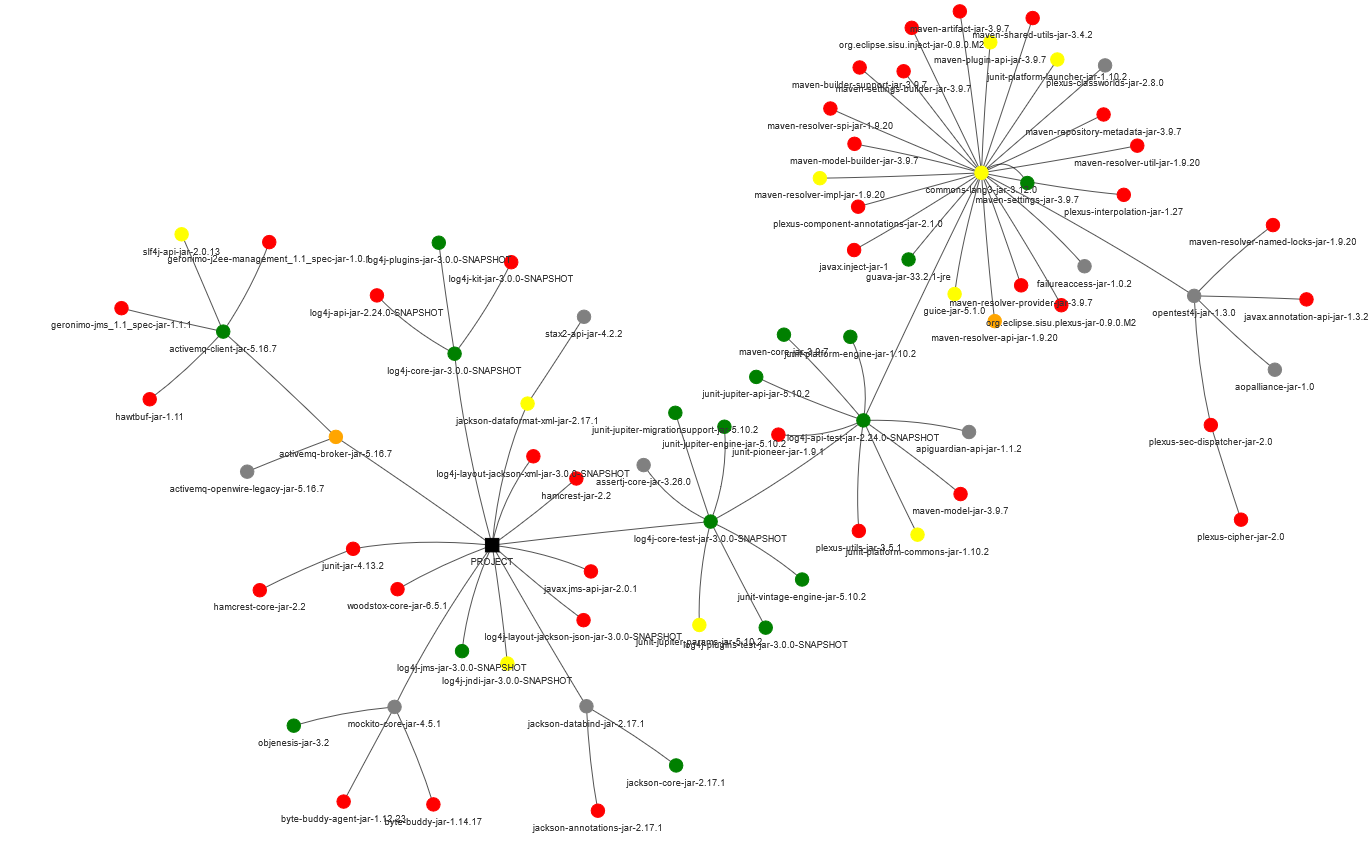
\includegraphics[width=1\linewidth]{image.png}
    \caption{Dependency Tree Results With Risk Levels Colour Coded} 
\end{figure}

Figure 1 shows a final dependency tree with colour-coded risk evaluations of each of the dependencies. This figure was based on a user configuration of two vulnerabilities being acceptable and 70 being the minimum number of commits per month as acceptable. 


\section{Results \& Evaluation}
To evaluate the algorithm we used a number of different maven projects with different dependencies. We made sure to use some projects that were discussed above in the case studies section. We used a Log4j maven sample project. 

We found that the project activity predictions generally performed a lot better than the vulnerability CVE data - presumably due to a lack of data in the NVD databases (which can in some cases mean no vulnerabilities - a good thing). A lot of the dependencies were also grouped in the same projects on GitHub which meant that there was only the need to calculate the prediction for these once. An issue we ran into was that there was no way of automatically using an API to find the GitHub projects of the dependencies - this meant we had to manually go through each of the dependency trees and find the project URLs on GitHub which does not bode well for scaling the project up for larger Maven projects. 

For the evaluation of the predictions in this project, we used the commonly used metrics: Mean absolute percentage error (MAPE), mean absolute error (MAE), and root mean squared error (RMSE). 

\section{Conclusions \& Further Work}
For the purpose of this paper, we focused on examining Maven dependency trees which are primarily used for Java projects. Further work could be done to examine other package manager dependency trees such as \textit{PyPI} for Python, \textit{NPM} for JavaScript, and \textit{Conan} for C. 

\printbibliography

\appendices
\section{Graphs}

\ifCLASSOPTIONcaptionsoff
  \newpage
\fi

\end{document}